\begin{flushright} {\tiny {\color{gray} (tikz\_quadrature\_idef2.tex)}} \end{flushright}
%~~~~~~~~~~~~~~~~~~~~~~~~~~~~~~~~~~~~~~~~~~~~~~~~~~~~~~~~~~~~~~~~~~~~~~~~~~~~~~~~~~~~~~~~~~~~~~~~~~


\begin{center}
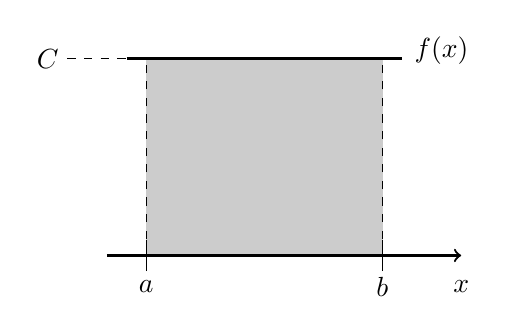
\begin{tikzpicture}
%\draw[step=0.5cm,gray,very thin] (0,0) grid (7,5); 
\draw[fill=gray!20,gray!40] (1,1)--(4,1)--(4,3.5)--(1,3.5)--cycle;
\draw [thick,->] (0.5,1) -- (5,1);
\node[] at (1,0.6) {$a$};
\node[] at (4,0.6) {$b$};
\node[] at (5,0.6) {$x$};
\draw [-] (1,0.8) -- (1,1.2);
\draw [-] (4,0.8) -- (4,1.2);
\draw [dashed] (1,1) -- (1,3.5);
\draw [dashed] (4,1) -- (4,3.5);
\draw[very thick] (0.75,3.5) --(4.25,3.5);
\node[] at (4.75,3.6) {$f(x)$};
\draw [dashed] (0,3.5) -- (4,3.5);
\node[] at (-0.25,3.5) {$C$};
\end{tikzpicture}
\end{center}




